\documentclass{article}
% --- watermark (auto-inserted) ---
\usepackage{xcolor}
\usepackage{xfp}% \fpeval; in the kernel since 2022, harmless on older LaTeX
\usepackage{draftwatermark}
\newlength{\watermarkTextWidth}
\AddToHook{begindocument/end}{%
  \SetWatermarkText{\normalfont Generated by The Agentic Scientist}%
  \SetWatermarkFontSize{10pt}%
  \SetWatermarkLightness{0.85}%
  \settowidth{\watermarkTextWidth}{\normalfont\fontsize{10pt}{12pt}\selectfont Generated by The Agentic Scientist}%
  \edef\watermarkScale{\fpeval{0.8 * sqrt(\paperwidth**2 + \paperheight**2) / \watermarkTextWidth}}%
  \edef\watermarkAngle{\fpeval{atand(\paperheight/\paperwidth)}}%
  \SetWatermarkScale{\watermarkScale}%
  \SetWatermarkAngle{\watermarkAngle}%
}
% --- end watermark ---

\usepackage{iclr2026_conference,times}
\usepackage{amsmath,amssymb,booktabs,graphicx,subcaption,longtable}
\usepackage{hyperref,url}
\title{Response Ceilings and Targeted Investment\\in Multitask Leaderboards}
\author{}
\newcommand{\cost}{K}
\newcommand{\eps}{\varepsilon}
\begin{document}
\maketitle

\begin{abstract}
Multitask leaderboards compress heterogeneous scores into a single ranking, creating incentives to improve selected tasks. Does replacing the mean with a median make attaining first place more expensive? We study this question under a transparent counterfactual: only a target model changes, each selected score closes a specified fraction of its remaining headroom, and investment counts selected task coordinates. Public HELM and Open LLM score panels permit comparisons of mean, conventional median, and symmetric trimmed mean. On fixed, jointly attainable cohorts in the six-task panel, exact minimum-support comparisons reverse between half and full headroom: median-minus-mean support fractions range from $-0.130$ to $-0.069$ at half headroom and from $+0.127$ to $+0.157$ at full headroom across sampling seeds. Attainability also differs substantially across rules. Larger subject panels yield exact mean costs but only bounded costs for order-statistic rules. Thus aggregation resistance is conditional on response ceilings, target selection, and certificate strength. These are score-space sensitivity results, not measured training costs or evidence of real contamination effects.
% @evidence[[derived/summary.json#central]]
\end{abstract}

\section{Introduction}
Multitask benchmarks make model comparison manageable by replacing a vector of task scores with an overall ranking. Their breadth is valuable: knowledge, instruction following, and reasoning need not improve together. But this compression also defines incentives. A developer interested in one model's position may concentrate effort on selected benchmark components rather than improving uniformly. The resulting question is not merely whether rankings change when a task is added or removed. It is how much targeted change to an existing score vector is sufficient to move a fixed target above every rival.

It is tempting to regard an order-statistic aggregator as intrinsically more resistant to concentrated investment than an arithmetic mean. The mean responds to every coordinate, whereas the median depends on central values and a trimmed mean discards tails. This intuition does not by itself answer the ranking question. Raising a weak score can have substantial effect on the mean but none on the median until the score crosses a central rank. Conversely, a median threshold may be reachable by modifying a relatively small set of central coordinates, while a mean threshold still requires improvement spread across many tasks. The permitted magnitude of each change is therefore part of the question, not an incidental nuisance parameter.

We formalize investment as the number of task coordinates receiving a bounded target-only uplift. The model is deliberately agnostic about the training intervention that might produce it. It asks a reproducible question about public score geometry with explicit ceilings and fixed competitors. We compare arithmetic mean, conventional median, and symmetric trimmed mean on public HELM subject scores and Open LLM task scores. A separate BBH subtask sensitivity check is kept distinct from the primary panels. These are different resolutions of evaluation, not interchangeable units of real-world training expense.
% @evidence[[source_evidence/downstream/program/src/program.py#L16-L28]]

Our central observation is a conditional ordering reversal. Holding the target cohort fixed within each sampling seed, the median requires less support on average than the mean at half headroom, but more at full headroom. This comparison uses exact costs on the six-task panel. It is not inferred from a mixture of successful and unsuccessful targets, or from heuristic solutions on larger panels. Alongside this contrast, we report all-target attainability, support intervals where exactness is unavailable, and matched selection-policy comparisons.
% @evidence[[derived/summary.json#central]]

The contributions are an explicit, implementable investment definition; an exact matched-cohort demonstration of response-dependent aggregation ordering; and an evidence-strength-aware comparison that separates attainability, minimum costs, and feasible upper bounds. We do not propose a new optimizer or infer an isolated component effect from uncontrolled changes. The main implication is methodological: an aggregation rule should not be described as resistant to targeted investment without specifying the response model and which cost statements are actually certified.

\begin{figure}[t]
\centering
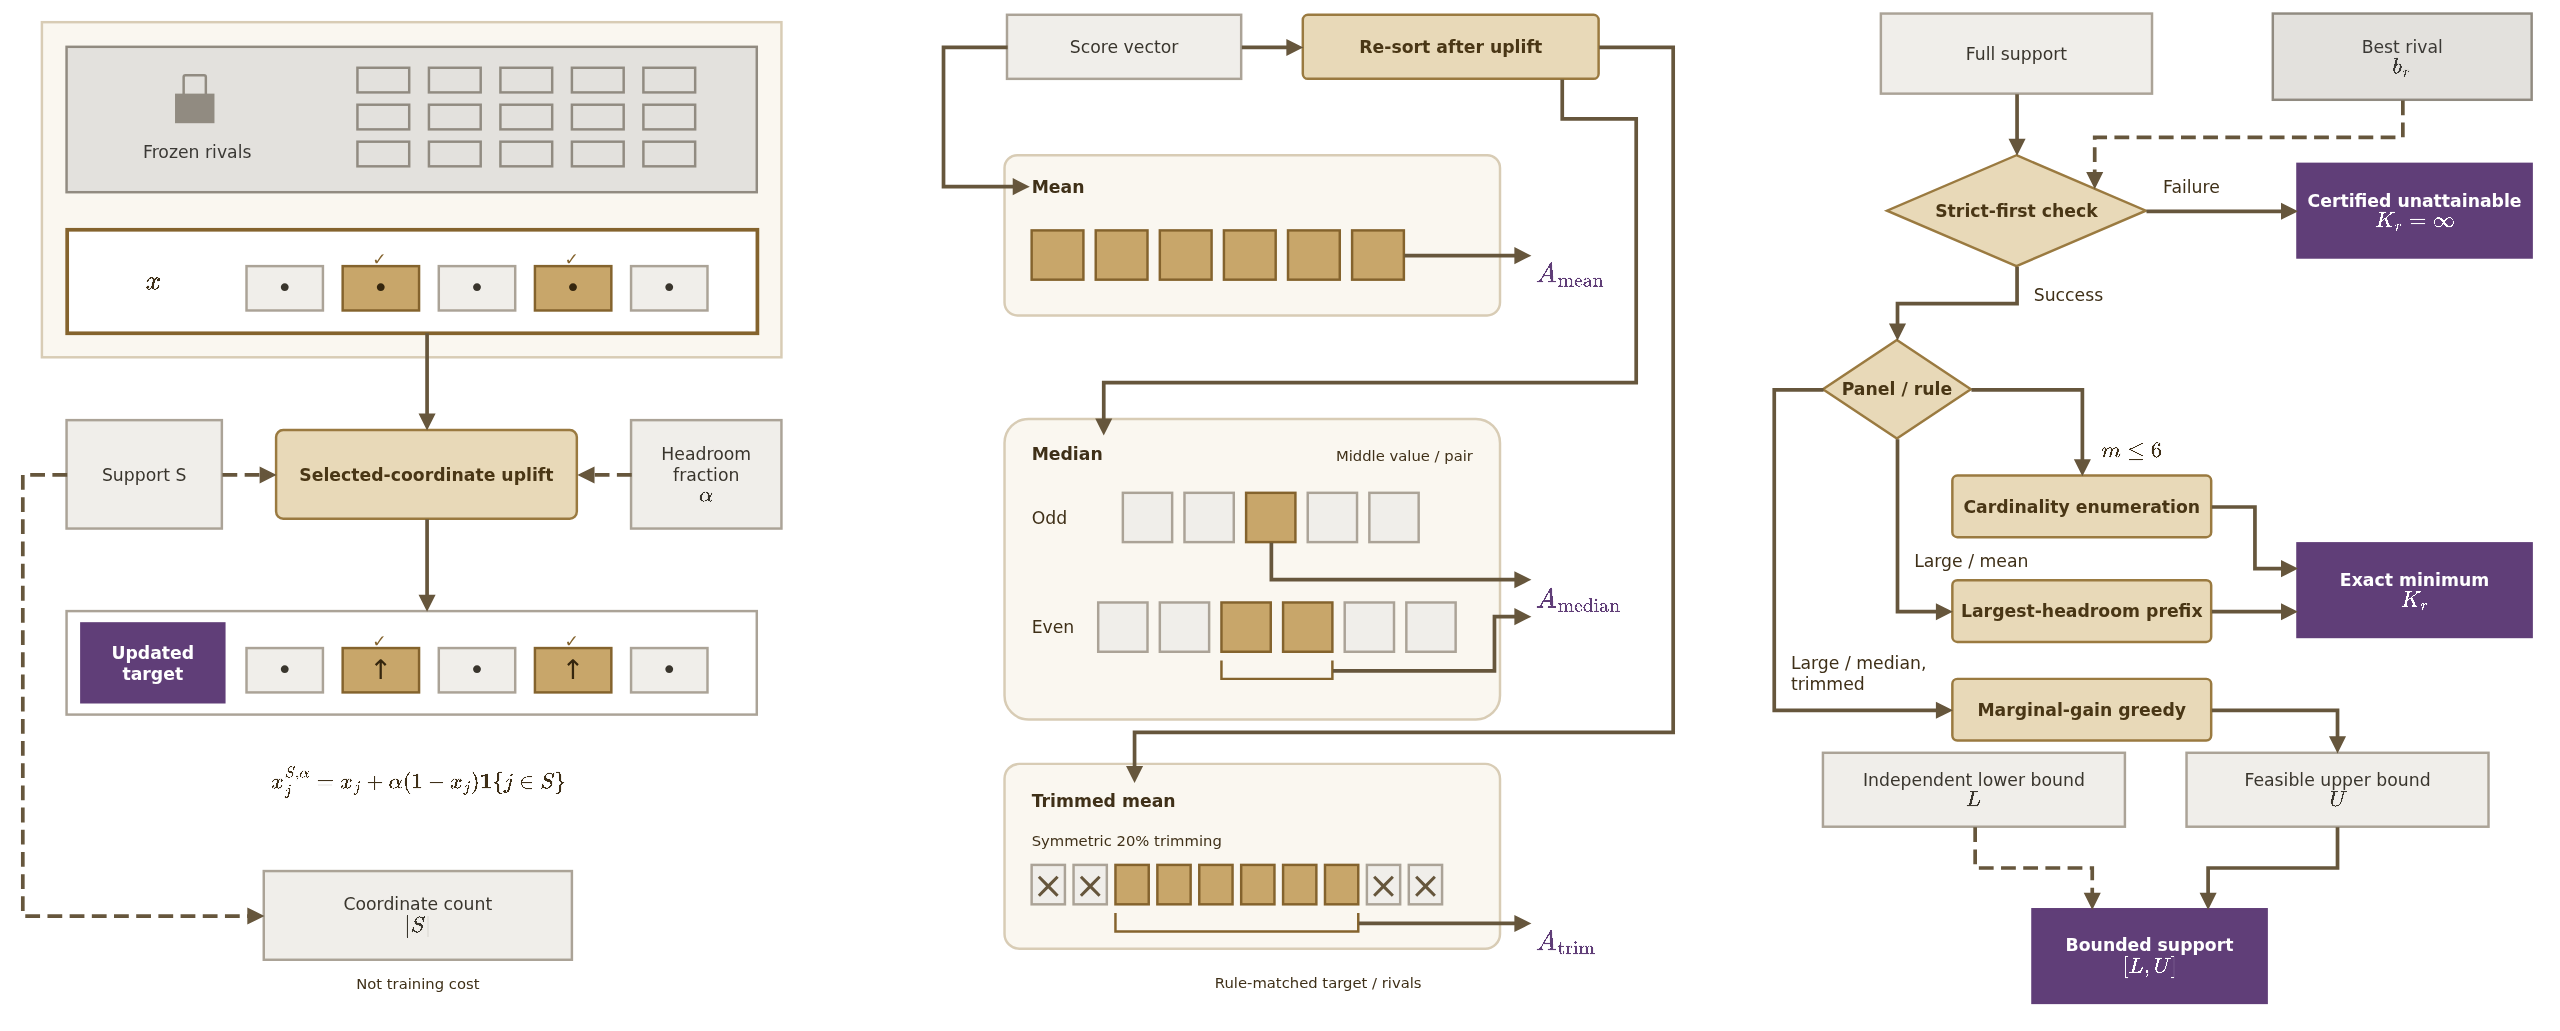
\includegraphics[width=\linewidth]{figures/investment_overview.png}
\caption{The studied counterfactual: modify only selected target coordinates, hold rivals fixed, and compare aggregation conditions. The outcome is an exact minimum support, certified unattainability, or a lower--upper support interval. No model training is represented.}
\label{fig:overview}
\end{figure}

\section{Related Work}
\paragraph{Evaluation breadth and benchmark composition.}
MMLU evaluates knowledge across subjects \citep{MMLU}; HELM emphasizes broad, transparent evaluation across scenarios and metrics \citep{HELM}. BIG-bench and BBH characterize diverse tasks and difficult reasoning settings \citep{BIGBench,BBH}. The six-task panel studied here combines instruction following \citep{IFEval}, challenging mathematics \citep{MATH}, expert question answering \citep{GPQA}, narrative reasoning \citep{MuSR}, and knowledge-oriented reasoning \citep{MMLUPro}, alongside BBH. These source works explain the tasks' purposes; our empirical claims concern the pinned score snapshots, not a replication of their original experiments. The benchmark-lottery perspective emphasizes that relative performance depends on benchmark choices \citep{Lottery}. We instead hold task membership fixed in the principal comparison and vary the aggregation rule and allowed target response.

\paragraph{Aggregation and statistical robustness.}
\citet{SocialChoice} interpret tasks as voters and evaluation as social aggregation. Our comparison uses cardinal score summaries rather than implementing their ordinal voting framework. Classical robust estimation studies sensitivity to contamination of observations \citep{Huber}. Resistance of a location estimate to contamination is not the same as support needed to exceed a rival's aggregation threshold under bounded upward changes. In particular, the target's order statistics and the rival threshold both matter here. We make no claim that the familiar mean, median, trimmed mean, exhaustive enumeration, or greedy policies are new.

\paragraph{Validity beyond a published score.}
Benchmark leakage and rephrased contamination motivate taking strategic score changes seriously \citep{Cheater,Rephrased}, but do not establish our assumed response law. Behavioral testing \citep{CheckList}, truthfulness evaluation \citep{TruthfulQA}, replication on fresh test sets \citep{ImageNetReplication}, and underspecification \citep{Underspecification} each illustrate a distinct reason not to equate one aggregate with general capability. Dataset and model documentation support stating intended uses and limitations \citep{Datasheets,ModelCards}. We follow that principle by distinguishing a hypothetical score intervention from observed training.

\paragraph{Comparisons and uncertainty.}
Comparisons across datasets require attention to the experimental unit \citep{Demsar}, and selection itself can bias performance evaluation \citep{Cawley}. Accordingly, our cross-rule reversal is descriptive and conditional on the observed snapshots and a post-selected framing. Recorded bootstrap intervals \citep{Efron} concern paired selection policies, not the reversal hypothesis. The reproduction environment specifies NumPy and SciPy \citep{NumPy,SciPy}; the summaries use NumPy arrays.
% @evidence[[source_evidence/evaluation/requirements.txt]]

\section{Method}
\subsection{Problem setup and response model}
Let $X\in[0,1]^{n\times m}$ be a public score matrix, with one row per evaluated model and one coordinate per task. Fix a target row $t$, its score vector $x=X_t$, and all other rows as rivals. For support $S\subseteq\{1,\ldots,m\}$ and headroom fraction $\alpha$, define
\begin{equation}
 x^{S,\alpha}_j=x_j+\alpha(1-x_j)\,\mathbf{1}\{j\in S\}.
 \label{eq:response}
\end{equation}
All selected coordinates receive the same fraction of remaining headroom. Unselected scores and all rival scores are unchanged. The evaluated ceilings are $\alpha\in\{0.25,0.5,1\}$. Full headroom allows a selected score to reach one; it is an optimistic stress condition, not an empirical prediction. Let $A_r$ denote aggregation rule $r$ and
\begin{equation}
 b_r=\max_{i\ne t} A_r(X_i),\qquad
 \cost_r(x,\alpha)=\min_S\{|S|:A_r(x^{S,\alpha})>b_r+\eps\},
 \label{eq:cost}
\end{equation}
where $\eps=10^{-10}$ implements strict first place. If no support wins, $\cost_r=\infty$. The normalized investment is $\cost_r/m$ when attainable. A tie does not count as first place.
% @evidence[[source_evidence/downstream/program/src/program.py#L16-L28]]
% @evidence[[paper_data.json#/final_evaluation/evaluation_evidence/episodes]]

This is an equal-coordinate cost model: intervening on a broad evaluation task and on a narrow subject each costs one within its own panel. Consequently, normalized support compares concentration within panels, not absolute work across datasets. It does not measure examples, money, accelerator time, or achievable learning gains. The assumptions exclude spillover, negative transfer, rivalry responses, and heterogeneity in the amount of work required to close headroom. Total score lift is available as a secondary diagnostic, but cannot calibrate those omitted quantities.

\subsection{Aggregation conditions and design rationale}
For sorted target values $z_{(1)}\le\cdots\le z_{(m)}$, the mean is $m^{-1}\sum_j z_j$. The conventional median takes the central order statistic for odd $m$ and averages the central pair for even $m$. The trimmed mean removes $q=\lfloor m/5\rfloor$ values from each end and averages the remaining $m-2q$. Tasks otherwise have equal weight. In the six-task panel this removes one value at each end, whereas on the subject panel trimming removes eleven at each end.
% @evidence[[source_evidence/downstream/program/src/program.py#L70-L79]]

The research question is whether the relative minimum support for two rules changes with $\alpha$. The mechanistic rationale is rank dependence: the mean rewards every positive uplift immediately; median and trimming rewards depend on where altered coordinates fall after sorting. Changing $\alpha$ changes which ranks a coordinate can reach. It also changes each rule's attainable set. There is therefore no reason to interpret a difference computed only on currently successful targets as a pure cost difference without controlling the cohort. We assess response-dependent ordering directly, without attributing it to a new selection component.

Within any fixed rule and target, increasing $\alpha$ cannot worsen attainability or increase the true minimum support: every coordinate and all three aggregators are monotone. This property does not constrain the sign of the difference between two rules' costs. A reversal of that difference is compatible with falling costs under both rules. Our primary contrast is the average median-minus-mean normalized support on targets attainable under both rules at both compared ceilings.

\subsection{Exact solutions, feasible witnesses, and bounds}
The frozen procedure begins by testing the full support. Since every allowed change is nonnegative and aggregation is coordinatewise monotone, failure of the full support certifies unattainability. This certificate is distinct from failure of a limited search. For a panel of at most six coordinates, supports are enumerated by cardinality, with deterministic semantic task-ID ordering. The first winning cardinality is exact. Thus every attainable primary six-task result used for the central contrast is a minimum-support result, not merely a successful heuristic plan.
% @evidence[[source_evidence/downstream/program/src/program.py#L99-L117]]
% @evidence[[derived/summary.json#central]]

For the mean on larger panels, sort headrooms $h_j=1-x_j$ from largest to smallest. Writing $h_{[j]}$ for this ordering, the minimum is the smallest $k$ satisfying
\begin{equation}
 \frac{1}{m}\sum_j x_j+\frac{\alpha}{m}\sum_{j=1}^k h_{[j]}>b_{\mathrm{mean}}+\eps.
 \label{eq:mean}
\end{equation}
No size-$k$ set can have greater summed headroom than this prefix, so a shorter failing prefix excludes all shorter supports. This explains exactness without invoking an unobserved solver behavior. Ties are resolved by semantic task identity.
% @evidence[[source_evidence/downstream/program/src/program.py#L118-L125]]

For larger median and trimmed panels, the procedure greedily adds the coordinate maximizing the immediate updated aggregate, again breaking ties by semantic task identity. It stops at a verified strict-first support. Its size is an upper bound $U$, not necessarily $\cost_r$. Independently computed conservative lower bounds $L$ yield $L\le\cost_r\le U$. The reported $L$ is the evaluator's verified reference bound, not a claim that the greedy procedure computes an exact optimum. Mean costs and exhaustive small-panel costs collapse to points. Unattainable cases have no finite support interval; the machine-readable out-of-range sentinel is never plotted as an investment cost.
% @evidence[[source_evidence/downstream/program/src/program.py#L126-L137]]
% @evidence[[source_evidence/evaluation/evaluate_final.py#L761-L789]]
% @evidence[[source_evidence/evaluation/evaluate_final.py#L873-L925]]

\subsection{Public score panels and experimental protocol}
The primary panels are HELM MMLU release v1.13.0 with 57 subject coordinates and the pinned Open LLM contents snapshot \citep{OpenLLMContents} with six raw-score coordinates: IFEval, BBH, MATH level 5, GPQA, MuSR, and MMLU-Pro. The official dataset card distinguishes the six fields labelled \texttt{Raw}, used here, from their parallel display-score fields. The snapshots were acquired on 2026-11-17. The extracted records preserve original rows and settings; completeness and finite scores in the unit interval are required. These scores are not standardized effect sizes or observations from a homogeneous new evaluation. Source versions, checksums, filtering, and normalization are recorded in the supplementary reproduction specification.
% @evidence[[source_evidence/data/manifest.json]]
% @evidence[[source_evidence/data/records.json]]
% @evidence[[literature/OpenLLMContents.json#inspected_fields]]

Model aliases, normalized raw components, and score-map identities are grouped before partitioning the source records. The final evaluation uses a frozen, content-separated partition rather than a newly trained model. Within each family, rows tied for the lead under any studied rule are excluded from target selection. Remaining rows are sorted by mean score and divided into 24 bands; one target per band is sampled using each seed in $\{1009,1013,1019\}$. All rivals in the corresponding frozen pool remain visible. Each target is evaluated under every rule and ceiling, providing paired decisions rather than independently sampled rule-specific targets. Seeds vary target sampling, not model training.
% @evidence[[source_evidence/evaluation/evaluate_final.py#L614-L687]]
% @evidence[[derived/summary.json#seeds]]

The evaluator checks returned supports against the supplied matrix and accepts exactness only when independently supported. The ordinary primary cases define the reported target attainment rate: a verified strict-first support with a supported claim, divided by all primary targets in that cell. Constant-ceiling, zero-response, joint column-permutation, and reset-replay checks test specific consistency properties. Replay carries no statistical weight. The completed frozen evaluation satisfies its recorded qualification requirements; this does not certify generalization outside the snapshots or validate unverified auxiliary diagnostics.
% @evidence[[source_evidence/data/manifest.json#protocol_policy]]
% @evidence[[paper_data.json#/final_evaluation/status]]
% @evidence[[paper_data.json#/final_evaluation/outcome]]

\subsection{Comparators, conditioning, and uncertainty}
Matched selection comparators are no intervention, a seeded random coordinate order, and the marginal-aggregate greedy policy. These are policies on the same target, panel, rule, and ceiling, not component ablations. For policy comparisons, define penalized effort $E=|S|/m$ for a verified successful support and $E=1$ otherwise. Assigning one to nonattainment is a reporting convention, not an observed minimum cost. Support plots instead condition on joint attainability and show genuine finite bounds.
% @evidence[[source_evidence/evaluation/evaluate_final.py#L790-L818]]
% @evidence[[source_evidence/evaluation/evaluate_final.py#L873-L925]]

The central comparison keeps a fixed cohort per seed across both rules and both ceilings. The three-rule support plots use the within-ceiling joint cohort, which may differ across ceilings; seed means receive equal weight. We show individual seed summaries rather than inventing a population confidence interval. Existing policy intervals use 200 paired cluster resamples with resampling seed 48271 and percentile endpoints at 95\%. They condition on the fixed snapshots and rival pools. They do not test differences between aggregation rules. Overlapping targets or related models across seeds further preclude treating these as independent training replications.
% @evidence[[source_evidence/evaluation/evaluate_final.py#L1046-L1068]]
% @evidence[[derived/summary.json#paired_intervals]]

\section{Results}
\subsection{Exact investment ordering changes with the response ceiling}
On the primary six-task panel, the fixed cohorts jointly attainable under mean and median at half and full headroom contain 18, 17, and 17 targets for seeds 1009, 1013, and 1019, respectively. Figure~\ref{fig:exact} shows the paired difference
\begin{equation}
 D_s(\alpha)=\frac{1}{|C_s|}\sum_{t\in C_s}
 \frac{\cost_{\mathrm{median}}(X_t,\alpha)-\cost_{\mathrm{mean}}(X_t,\alpha)}{6}.
\end{equation}
The cohort $C_s$ is unchanged between panels. All included supports have exact minimum status backed by exhaustive selection. Therefore the comparison is about minimum investment in the specified model, not differences in heuristic success.
% @evidence[[derived/summary.json#central]]

\begin{figure}[t]
\centering
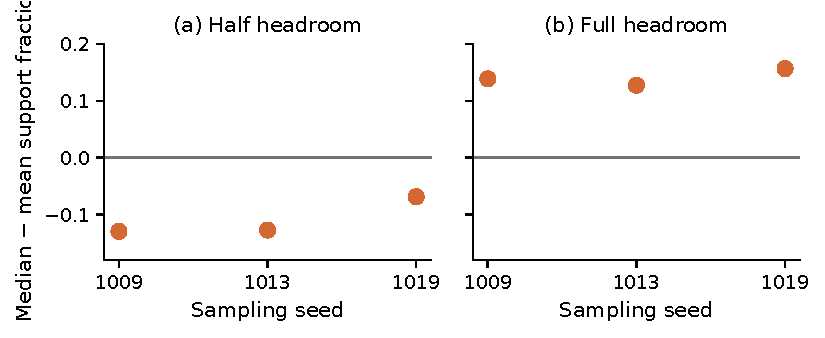
\includegraphics[width=\linewidth]{figures/exact_rule_contrast.pdf}
\caption{Exact paired contrast on fixed Open LLM cohorts. Negative values mean the median requires fewer modified coordinates on average. The same targets are retained at half and full headroom within each seed; cohort sizes are 18, 17, and 17. Points are descriptive seed summaries, not confidence intervals.}
\label{fig:exact}
% @evidence[[derived/summary.json#central]]
\end{figure}

At half headroom, $D_s$ is $-0.1296$, $-0.1275$, and $-0.0686$ in seed order. At full headroom it is $+0.1389$, $+0.1275$, and $+0.1569$. Thus the average ordering reverses in every sampled cohort: median support is lower at half headroom and higher at full headroom. This does not mean each target reverses, nor does it estimate how frequently reversal would occur in a new leaderboard. The contrast was selected descriptively during analysis of the recorded results and is not a preregistered hypothesis test.
% @evidence[[derived/summary.json#central]]

Holding the cohort fixed is important. At half headroom, some targets cannot win under one or both rules. Comparing the mean on all mean-attainable targets with the median on all median-attainable targets would conflate ranking resistance with selection of different models. Our fixed-cohort comparison removes that particular change in composition, while remaining conditional on joint attainability. Its claim is consequently narrower, but also cleaner: response ceilings can change rule ordering even without changing the compared targets.

\subsection{Attainability and support answer different questions}
Figure~\ref{fig:scope} includes all ordinary primary targets in its attainment panels. Each rule--ceiling cell contains 72 target decisions across the sampling seeds. On Open LLM, quarter headroom yields attainment for 11 targets under the mean, one under the median, and eight under trimming. At half headroom these counts are 65, 52, and 67; full headroom attains all 72 under every rule. A median can therefore have lower average cost on the jointly attainable cohort while excluding more targets overall. Neither quantity should be substituted for the other.
% @evidence[[derived/summary.json#grid]]

On HELM, quarter-headroom counts are nine, nine, and eight for mean, median, and trimming; half-headroom counts are 42, 42, and 41. All rules attain all 72 targets at full headroom. The low-ceiling nonattainment here is certified by the all-coordinate test. It is not a count of unresolved heuristic failures. These snapshots support a strong role for response magnitude, but do not identify the response magnitudes that actual post-training would achieve.
% @evidence[[derived/summary.json#grid]]

\begin{figure}[t]
\centering
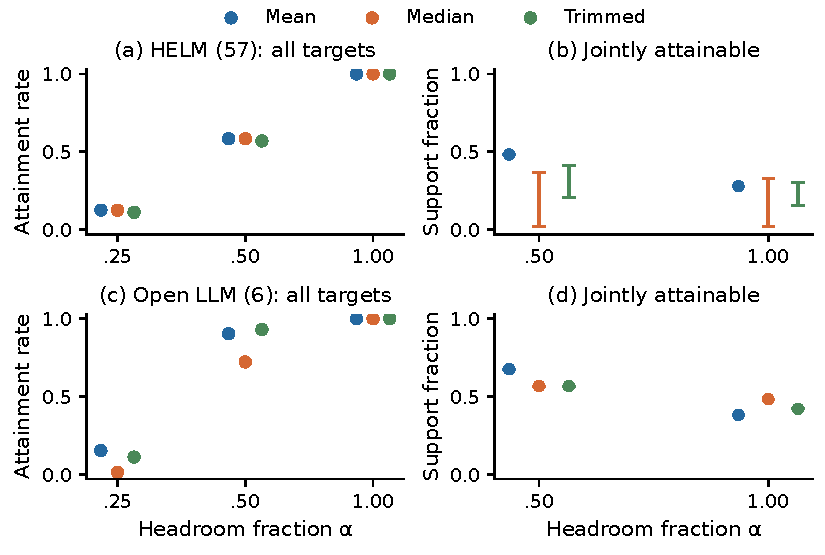
\includegraphics[width=\linewidth]{figures/attainability_and_support_scope.pdf}
\caption{Attainability and certificate scope. Left: all ordinary primary targets, with one strict-first definition throughout. Right: equal-seed average support bounds on targets attainable under all three rules at that ceiling. HELM cohort sizes are $(14,13,13)$ at half and $(24,24,24)$ at full headroom; Open LLM sizes are $(18,17,17)$ and $(24,24,24)$. Bars are certification ranges, not statistical intervals; points indicate exact costs. Unlike Figure~\ref{fig:exact}, right-panel cohorts can change across ceilings.}
\label{fig:scope}
% @evidence[[derived/summary.json#grid]]
% @evidence[[derived/summary.json#support]]
\end{figure}

The right panels expose the difference between exact and bounded evidence. On the HELM joint cohort at half headroom, the exact mean support fraction is $0.483$, while median and trimmed support intervals are $[0.018,0.364]$ and $[0.205,0.414]$. These averaged intervals lie below the exact mean cost on that cohort. This establishes a lower average cost than the mean there even without resolving the individual order-statistic optima. At full headroom, the mean cost is $0.279$, while median and trimming intervals are $[0.018,0.330]$ and $[0.153,0.304]$. These overlap the mean point, so a reversal of the large-panel minimum-cost ordering is not established. A feasible upper bound above the mean does not prove a higher minimum.
% @evidence[[derived/summary.json#support]]

On the six-task joint cohorts the intervals collapse. Half-headroom mean, median, and trimming costs are $0.676$, $0.568$, and $0.568$; the full-headroom values are $0.382$, $0.484$, and $0.421$. These within-ceiling summaries give context for the matched result, but they use different cohorts at the two ceilings. The primary reversal claim rests on Figure~\ref{fig:exact}, not on comparing these marginal averages.
% @evidence[[derived/summary.json#support]]

\subsection{Selection-policy comparisons do not imply optimizer novelty}
Table~\ref{tab:policies} compares matched policies at half headroom over all targets, using penalized effort. The frozen procedure ties marginal greedy for every HELM rule and for the six-task mean. This is expected from their shared selection behavior in these conditions. On the six-task median and trimmed mean, exhaustive selection attains smaller penalized effort than the recorded greedy policy. The distinction matters: marginal gain can fail to anticipate the benefit of a set of coordinates jointly changing an order statistic.
% @evidence[[derived/comparators.tex]]
% @evidence[[source_evidence/downstream/program/src/program.py#L109-L137]]

\begin{table}[t]
\centering
\caption{Matched policy comparison at half headroom. Lower penalized effort is better; nonattainment contributes one. Exact/witness denotes exhaustive selection on the six-task panel, sorted headroom for means, and a feasible greedy witness for larger order-statistic panels. Values average all targets with equal seed weights.}
\label{tab:policies}
\begin{tabular}{llrrrr}
\toprule
Panel & Rule & Exact/witness & Greedy & Random & None\\
\midrule
% BEGIN GENERATED comparators
HELM & Mean & 0.707 & 0.707 & 0.835 & 1.000 \\
HELM & Median & 0.639 & 0.639 & 0.780 & 1.000 \\
HELM & Trimmed & 0.670 & 0.670 & 0.819 & 1.000 \\
Open LLM & Mean & 0.764 & 0.764 & 0.822 & 1.000 \\
Open LLM & Median & 0.688 & 0.799 & 0.831 & 1.000 \\
Open LLM & Trimmed & 0.650 & 0.688 & 0.762 & 1.000 \\
% END GENERATED comparators
\bottomrule
\end{tabular}
% @evidence[[derived/comparators.tex]]
\end{table}

For example, the six-task median has penalized effort $0.688$ versus greedy $0.799$ and random $0.831$; trimming has $0.650$, $0.688$, and $0.762$. No intervention yields one throughout, because target selection excludes existing leaders. These are observed policy comparisons under the response model, not improvements over a distinct evaluated architecture or a new exact algorithm. They also do not license claiming an average attainable minimum of $0.688$: that statistic includes unsuccessful targets by construction.
% @evidence[[derived/comparators.tex]]

Recorded cluster-resampling intervals for the policy contrasts, together with the complete rule--ceiling grid, appear in Supplementary Information. The intervals retain the unit of resampling used by the evaluator and are not reassigned to the cross-rule contrast. No controlled component ablation supports a mechanistic attribution to a proposed optimization refinement. The measured exact-versus-greedy difference is sufficient for the limited selection-policy conclusion.
% @evidence[[derived/summary.json#paired_intervals]]

\subsection{Scope checks and limits of the evaluated evidence}
Auxiliary decisions include a six-coordinate HELM projection and a separately routed BBH panel with 24 recorded subtask coordinates. Open LLM auxiliary odd slots use BBH and even slots use the six-task family; those slots must not be interpreted as matched primary model identities. The BBH results are revision-matched but drawn from a distinct results snapshot, so matching model revisions does not establish identical evaluation settings. Their attainment and certificate counts are reported separately in the supplement, without pooling them into the primary findings.
% @evidence[[source_evidence/evaluation/evaluate_final.py#L718-L732]]
% @evidence[[source_evidence/data/manifest.json#reconciliation]]
% @evidence[[derived/auxiliary.tex]]

The final evaluation is completed and qualified, with recorded control pass fraction $1.0$. Qualification concerns the evaluator's supported claims and specified consistency checks, not optimality of every large-panel witness or unbiasedness of the post-selected scientific framing. Candidate-supplied diagnostics remain unverified; our measurements use recorded evaluator decisions and inspectable source instead. There is no failed final qualification to reinterpret as a performance result. The absence of a qualifying alternative in development does not invalidate the completed frozen comparison, and neither fact establishes general superiority.
% @evidence[[paper_data.json#/final_evaluation/status]]
% @evidence[[paper_data.json#/final_evaluation/outcome]]
% @evidence[[paper_data.json#/final_evaluation/metrics/control_pass_rate]]
% @evidence[[paper_data.json#/final_evaluation/evaluation_evidence/candidate_diagnostics_trust]]

\section{Discussion and Limitations}
\paragraph{What investment means.}
Counting coordinates isolates how aggregation rewards concentration, but it is not a training-production model. A unit of investment in a broad reasoning benchmark is not commensurate with a unit in an individual knowledge subject. Even within a panel, two tasks may have very different data access costs, learning curves, or contamination risks. Equal fractional headroom is useful because it is transparent, monotone, and bounded by the score range. It is not justified as a fitted account of any particular training process. Conclusions should therefore be stated conditionally: \emph{if} these coordinate responses are available, this support suffices or is necessary.

\paragraph{What the reversal does and does not show.}
The result rules out treating the observed mean--median ordering as independent of the permitted response ceiling in this setting. It does not establish a universal ordering, a population reversal frequency, or a theorem that medians are generally easy to manipulate. Changing the rival pool changes the threshold; changing the target distribution changes which costs are averaged. The fixed-cohort design controls one source of composition bias, but conditions away targets that fail under either rule at half headroom. Attainment plots are essential precisely because those excluded targets are substantively important. Likewise, the three-rule support cohorts serve a different question from the two-rule fixed cohorts and cannot be silently interchanged.

\paragraph{Data and inference limits.}
Snapshots include heterogeneous model settings and related model families. Content-based partitioning reduces literal overlap but does not ensure independence of model ancestry, shared training data, or benchmark familiarity. Seeds sample frozen rows rather than generate new learning outcomes. The framing was chosen after inspecting the recorded decisions; an independent snapshot or preregistered comparison would be needed for stronger confirmatory claims. Existing policy bootstrap intervals quantify only their conditional resampling variability. They omit uncertainty in benchmark scores, data acquisition, response calibration, rival selection, and the choice of framing.

\paragraph{Certificates and practical use.}
The larger-panel order-statistic results should be used as intervals. Weak lower bounds leave substantial uncertainty even when a returned support wins, and the final consistency checks do not close that uncertainty. The HELM half-headroom comparison is informative because the upper bounds already lie below the mean cost; the full-headroom comparison is unresolved because the intervals overlap. This asymmetric interpretation preserves evidence that is genuinely available without turning unresolved optima into measured losses. A leaderboard designer using this analysis should inspect attainability and certificate width together, and should test response assumptions rather than choosing an aggregator from one marginal cost summary.
% @evidence[[derived/summary.json#support]]

Finally, public accessibility does not settle redistribution rights. No separate license for the score data was identified in the acquisition manifest. Code and model licenses do not automatically license score extracts. The reproducibility materials preserve source locations and checksums, but public redistribution requires a separate permissions review. The study neither trains a model on benchmark data nor provides evidence that a model's real benchmark performance was strategically altered.
% @evidence[[source_evidence/data/manifest.json#license_assessment]]

\section{Conclusion}
Targeted investment in a multitask leaderboard depends jointly on the aggregation rule and on what each selected task can gain. Under a bounded target-only response model, exact six-task results show that mean--median minimum-support ordering reverses between half and full headroom on the same jointly attainable targets. The observation survives each recorded target-sampling seed, but remains a descriptive result for frozen public score panels rather than a claim about independent training replications or new leaderboards.
% @evidence[[derived/summary.json#central]]

Separating attainability from support cost changes the interpretation: a rule can require less investment among shared successful targets while excluding more targets overall. Separating exact optima from feasible witnesses matters equally. Subject-level results establish useful bounds, including a half-headroom comparison, but do not establish the same full-headroom minimum-cost reversal. The defensible takeaway is not that one aggregator is inherently best. It is that claims about resistance to targeted investment require an explicit response ceiling, a declared target cohort, and a clear account of certificate strength. Calibrating these score-space changes against observed training responses remains necessary before translating the results into practical expenditure or benchmark-governance guarantees.

\clearpage
\bibliography{references}
\bibliographystyle{iclr2026_conference}

\clearpage
\appendix
\section{Supplementary Information}
\subsection{Source-level method evidence and reproduction}
The evaluated implementation is inspectable at
\path{source_evidence/downstream/program/src/program.py}.
Lines 70--79 define aggregation; lines 83--108 form the rival threshold and full-support test; lines 109--117 enumerate small supports; lines 118--125 solve larger means by headroom; and lines 126--137 construct larger order-statistic witnesses. The entrypoint is declared by the adjacent \path{program_spec.toml}. The selected and reference source copies are identical; no implementation change is inferred from a hash or a family label. The evaluator's \path{source_evidence/evaluation/evaluate_final.py}, lines 761--789 and 873--925, supplies reference bounds and independently verifies returned supports. These locations support the implementation description, not merely its provenance identity.
% @evidence[[source_evidence/downstream/program/src/program.py]]
% @evidence[[source_evidence/downstream/baseline/src/program.py]]
% @evidence[[source_evidence/evaluation/evaluate_final.py]]

All quantitative figures and tables in this manuscript are regenerated by
\path{scripts/build_paper_artifacts.py} from the existing final records in
\path{paper_data.json}; it does not rerun the evaluation. It writes
\path{derived/summary.json}, the two quantitative figure groups, the main policy table, and the extended tables below, with input-linked provenance sidecars. The overview is reserved for the separate synchronous concept-figure renderer and contains no empirical measurements. The commands, environment record, and acquisition instructions are in \path{REPRODUCIBILITY.md}. Scientific-evidence references in source comments are intentionally nonprinting.
% @evidence[[scripts/build_paper_artifacts.py]]
% @evidence[[figure_manifest.json]]

\subsection{Snapshot provenance and evaluation settings}
The HELM source is the public MMLU release v1.13.0 under
\url{https://storage.googleapis.com/crfm-helm-public/}.
The Open LLM contents revision is
\texttt{9c09a7cae43334062a82cb164f2ef255013dafa2}; the distinct results revision used for BBH is
\texttt{aa81ecc38fdc5708254b833923368970efdf5ef5}.
Acquisition was recorded on 2026-11-17. The extracted-record SHA-256 is
\texttt{d80abb1b13c6962e15f04d9794fc18fcf39e91cf7c79c679e233d3031f934398}.
Per-source checksums, raw source locations, and license uncertainty are preserved in \path{source_evidence/data/manifest.json}. These revisions identify inputs; they do not establish uniform evaluation conditions.
% @evidence[[source_evidence/data/manifest.json]]

Normalization applies Unicode NFKC, collapses whitespace, normalizes line endings, and recursively sorts canonical JSON, with integer-valued floats canonicalized as integers. Missing and null values remain distinct. Alias, normalized-component, and score-map identity links define connected components before deterministic content partitioning. The underlying raw source rows retain evaluation-setting fields. Matching a BBH model revision is required, but does not prove equivalence between contents and results evaluations. BBH is retained only with complete recorded subtask panels and is reported independently.
% @evidence[[source_evidence/data/manifest.json#normalization]]
% @evidence[[source_evidence/data/manifest.json#split]]
% @evidence[[source_evidence/evaluation/evaluate_final.py#L614-L669]]

The evaluator uses CPU-only computation, a final wall allowance of 1800 seconds, and matched per-method reservations of ten productive seconds per episode, including transfer and output within that reservation. Decisions carry an advisory node budget of 20000; the frozen reference selection is determined by its explicit enumeration, sorting, and greedy code rather than by a novel node-limited search. Software requirements pin NumPy 2.2.6, SciPy 1.15.3, PyArrow 19.0.1, and Matplotlib 3.10.3. The paper-analysis environment is separately recorded to distinguish manuscript regeneration from the original evaluation.
% @evidence[[source_evidence/evaluation/evaluate_final.py#L39-L54]]
% @evidence[[source_evidence/evaluation/evaluate_final.py#L731-L732]]
% @evidence[[source_evidence/evaluation/requirements.txt]]
% @evidence[[derived/environment.json]]

\subsection{Complete primary comparison grid}
Table~\ref{tab:grid} reports every primary rule--ceiling cell. Fractions count target decisions, not unique independent model families. Penalized effort is defined in the main text and must not be interpreted as cost conditional on success. All nonattaining ordinary primary cases in these records are certified unattainable rather than unresolved.
% @evidence[[derived/summary.json#grid]]
\begin{table}[h]
\centering
\caption{Full primary grid. Attainment denominators include all sampled target decisions. Effort columns include the nonattainment penalty.}
\label{tab:grid}
\begin{tabular}{lllrrrr}
\toprule
Panel & Rule & $\alpha$ & Attained & Exact/witness & Greedy & Random\\
\midrule
% BEGIN GENERATED full_grid
HELM & Mean & 0.25 & 9/72 & 0.937 & 0.937 & 0.973 \\
HELM & Median & 0.25 & 9/72 & 0.891 & 0.891 & 0.931 \\
HELM & Trimmed & 0.25 & 8/72 & 0.925 & 0.925 & 0.962 \\
HELM & Mean & 0.50 & 42/72 & 0.707 & 0.707 & 0.835 \\
HELM & Median & 0.50 & 42/72 & 0.639 & 0.639 & 0.780 \\
HELM & Trimmed & 0.50 & 41/72 & 0.670 & 0.670 & 0.819 \\
HELM & Mean & 1.00 & 72/72 & 0.279 & 0.279 & 0.469 \\
HELM & Median & 1.00 & 72/72 & 0.330 & 0.330 & 0.382 \\
HELM & Trimmed & 1.00 & 72/72 & 0.304 & 0.304 & 0.390 \\
Open LLM & Mean & 0.25 & 11/72 & 0.965 & 0.965 & 0.979 \\
Open LLM & Median & 0.25 & 1/72 & 0.993 & 0.993 & 1.000 \\
Open LLM & Trimmed & 0.25 & 8/72 & 0.951 & 0.951 & 0.975 \\
Open LLM & Mean & 0.50 & 65/72 & 0.764 & 0.764 & 0.822 \\
Open LLM & Median & 0.50 & 52/72 & 0.688 & 0.799 & 0.831 \\
Open LLM & Trimmed & 0.50 & 67/72 & 0.650 & 0.688 & 0.762 \\
Open LLM & Mean & 1.00 & 72/72 & 0.382 & 0.382 & 0.465 \\
Open LLM & Median & 1.00 & 72/72 & 0.484 & 0.484 & 0.512 \\
Open LLM & Trimmed & 1.00 & 72/72 & 0.421 & 0.421 & 0.456 \\
% END GENERATED full_grid
\bottomrule
\end{tabular}
% @evidence[[derived/full_grid.tex]]
\end{table}

\subsection{Conditional paired policy intervals}
The following table reproduces all recorded ordinary primary policy contrasts. Each row is exact/witness penalized effort minus comparator penalized effort. Negative values favor the frozen procedure. Clusters are the recorded alias/content groups; resampling is within a rule, ceiling, family, and seed. Percentile endpoints use 200 resamples, seed 48271. These are conditional 95\% intervals and are not multiple-comparison-adjusted discovery claims. A zero-width tie means identical recorded differences in that cell, not uncertainty-free performance on new data.
% @evidence[[derived/summary.json#paired_intervals]]
% @evidence[[source_evidence/evaluation/evaluate_final.py#L1046-L1068]]
\begin{longtable}{rlll lrr}
\caption{Recorded paired policy differences and conditional intervals.}\label{tab:intervals}\\
\toprule Seed & Panel & Rule & $\alpha$ & Comparator & Difference & Interval\\\midrule
\endfirsthead
\toprule Seed & Panel & Rule & $\alpha$ & Comparator & Difference & Interval\\\midrule
\endhead
% BEGIN GENERATED paired_intervals
1009 & HELM & Mean & 0.25 & Random & -0.040 & [-0.080, -0.012] \\
1009 & HELM & Mean & 0.25 & Greedy & +0.000 & [+0.000, +0.000] \\
1009 & HELM & Mean & 0.50 & Random & -0.127 & [-0.173, -0.087] \\
1009 & HELM & Mean & 0.50 & Greedy & +0.000 & [+0.000, +0.000] \\
1009 & HELM & Mean & 1.00 & Random & -0.194 & [-0.213, -0.171] \\
1009 & HELM & Mean & 1.00 & Greedy & +0.000 & [+0.000, +0.000] \\
1009 & HELM & Median & 0.25 & Random & -0.045 & [-0.099, +0.000] \\
1009 & HELM & Median & 0.25 & Greedy & +0.000 & [+0.000, +0.000] \\
1009 & HELM & Median & 0.50 & Random & -0.140 & [-0.213, -0.072] \\
1009 & HELM & Median & 0.50 & Greedy & +0.000 & [+0.000, +0.000] \\
1009 & HELM & Median & 1.00 & Random & -0.052 & [-0.066, -0.035] \\
1009 & HELM & Median & 1.00 & Greedy & +0.000 & [+0.000, +0.000] \\
1009 & HELM & Trimmed & 0.25 & Random & -0.034 & [-0.073, +0.000] \\
1009 & HELM & Trimmed & 0.25 & Greedy & +0.000 & [+0.000, +0.000] \\
1009 & HELM & Trimmed & 0.50 & Random & -0.147 & [-0.202, -0.081] \\
1009 & HELM & Trimmed & 0.50 & Greedy & +0.000 & [+0.000, +0.000] \\
1009 & HELM & Trimmed & 1.00 & Random & -0.090 & [-0.110, -0.073] \\
1009 & HELM & Trimmed & 1.00 & Greedy & +0.000 & [+0.000, +0.000] \\
1009 & Open LLM & Mean & 0.25 & Random & -0.014 & [-0.035, +0.000] \\
1009 & Open LLM & Mean & 0.25 & Greedy & +0.000 & [+0.000, +0.000] \\
1009 & Open LLM & Mean & 0.50 & Random & -0.049 & [-0.077, -0.021] \\
1009 & Open LLM & Mean & 0.50 & Greedy & +0.000 & [+0.000, +0.000] \\
1009 & Open LLM & Mean & 1.00 & Random & -0.076 & [-0.111, -0.049] \\
1009 & Open LLM & Mean & 1.00 & Greedy & +0.000 & [+0.000, +0.000] \\
1009 & Open LLM & Median & 0.25 & Random & -0.021 & [-0.083, +0.000] \\
1009 & Open LLM & Median & 0.25 & Greedy & +0.000 & [+0.000, +0.000] \\
1009 & Open LLM & Median & 0.50 & Random & -0.181 & [-0.243, -0.125] \\
1009 & Open LLM & Median & 0.50 & Greedy & -0.125 & [-0.167, -0.083] \\
1009 & Open LLM & Median & 1.00 & Random & -0.028 & [-0.049, -0.007] \\
1009 & Open LLM & Median & 1.00 & Greedy & +0.000 & [+0.000, +0.000] \\
1009 & Open LLM & Trimmed & 0.25 & Random & -0.021 & [-0.042, +0.000] \\
1009 & Open LLM & Trimmed & 0.25 & Greedy & +0.000 & [+0.000, +0.000] \\
1009 & Open LLM & Trimmed & 0.50 & Random & -0.139 & [-0.181, -0.097] \\
1009 & Open LLM & Trimmed & 0.50 & Greedy & -0.049 & [-0.076, -0.021] \\
1009 & Open LLM & Trimmed & 1.00 & Random & -0.042 & [-0.070, -0.014] \\
1009 & Open LLM & Trimmed & 1.00 & Greedy & +0.000 & [+0.000, +0.000] \\
1013 & HELM & Mean & 0.25 & Random & -0.028 & [-0.069, +0.000] \\
1013 & HELM & Mean & 0.25 & Greedy & +0.000 & [+0.000, +0.000] \\
1013 & HELM & Mean & 0.50 & Random & -0.121 & [-0.167, -0.074] \\
1013 & HELM & Mean & 0.50 & Greedy & +0.000 & [+0.000, +0.000] \\
1013 & HELM & Mean & 1.00 & Random & -0.183 & [-0.208, -0.161] \\
1013 & HELM & Mean & 1.00 & Greedy & +0.000 & [+0.000, +0.000] \\
1013 & HELM & Median & 0.25 & Random & -0.056 & [-0.121, +0.000] \\
1013 & HELM & Median & 0.25 & Greedy & +0.000 & [+0.000, +0.000] \\
1013 & HELM & Median & 0.50 & Random & -0.129 & [-0.207, -0.071] \\
1013 & HELM & Median & 0.50 & Greedy & +0.000 & [+0.000, +0.000] \\
1013 & HELM & Median & 1.00 & Random & -0.058 & [-0.076, -0.040] \\
1013 & HELM & Median & 1.00 & Greedy & +0.000 & [+0.000, +0.000] \\
1013 & HELM & Trimmed & 0.25 & Random & -0.036 & [-0.088, +0.000] \\
1013 & HELM & Trimmed & 0.25 & Greedy & +0.000 & [+0.000, +0.000] \\
1013 & HELM & Trimmed & 0.50 & Random & -0.154 & [-0.204, -0.094] \\
1013 & HELM & Trimmed & 0.50 & Greedy & +0.000 & [+0.000, +0.000] \\
1013 & HELM & Trimmed & 1.00 & Random & -0.087 & [-0.098, -0.077] \\
1013 & HELM & Trimmed & 1.00 & Greedy & +0.000 & [+0.000, +0.000] \\
1013 & Open LLM & Mean & 0.25 & Random & -0.014 & [-0.028, +0.000] \\
1013 & Open LLM & Mean & 0.25 & Greedy & +0.000 & [+0.000, +0.000] \\
1013 & Open LLM & Mean & 0.50 & Random & -0.056 & [-0.084, -0.028] \\
1013 & Open LLM & Mean & 0.50 & Greedy & +0.000 & [+0.000, +0.000] \\
1013 & Open LLM & Mean & 1.00 & Random & -0.069 & [-0.097, -0.042] \\
1013 & Open LLM & Mean & 1.00 & Greedy & +0.000 & [+0.000, +0.000] \\
1013 & Open LLM & Median & 0.25 & Random & +0.000 & [+0.000, +0.000] \\
1013 & Open LLM & Median & 0.25 & Greedy & +0.000 & [+0.000, +0.000] \\
1013 & Open LLM & Median & 0.50 & Random & -0.146 & [-0.195, -0.083] \\
1013 & Open LLM & Median & 0.50 & Greedy & -0.111 & [-0.153, -0.069] \\
1013 & Open LLM & Median & 1.00 & Random & -0.035 & [-0.062, -0.014] \\
1013 & Open LLM & Median & 1.00 & Greedy & +0.000 & [+0.000, +0.000] \\
1013 & Open LLM & Trimmed & 0.25 & Random & -0.028 & [-0.063, +0.000] \\
1013 & Open LLM & Trimmed & 0.25 & Greedy & +0.000 & [+0.000, +0.000] \\
1013 & Open LLM & Trimmed & 0.50 & Random & -0.097 & [-0.139, -0.062] \\
1013 & Open LLM & Trimmed & 0.50 & Greedy & -0.035 & [-0.063, -0.007] \\
1013 & Open LLM & Trimmed & 1.00 & Random & -0.021 & [-0.049, +0.000] \\
1013 & Open LLM & Trimmed & 1.00 & Greedy & +0.000 & [+0.000, +0.000] \\
1019 & HELM & Mean & 0.25 & Random & -0.042 & [-0.080, +0.000] \\
1019 & HELM & Mean & 0.25 & Greedy & +0.000 & [+0.000, +0.000] \\
1019 & HELM & Mean & 0.50 & Random & -0.135 & [-0.188, -0.089] \\
1019 & HELM & Mean & 0.50 & Greedy & +0.000 & [+0.000, +0.000] \\
1019 & HELM & Mean & 1.00 & Random & -0.193 & [-0.214, -0.175] \\
1019 & HELM & Mean & 1.00 & Greedy & +0.000 & [+0.000, +0.000] \\
1019 & HELM & Median & 0.25 & Random & -0.019 & [-0.057, +0.000] \\
1019 & HELM & Median & 0.25 & Greedy & +0.000 & [+0.000, +0.000] \\
1019 & HELM & Median & 0.50 & Random & -0.154 & [-0.235, -0.083] \\
1019 & HELM & Median & 0.50 & Greedy & +0.000 & [+0.000, +0.000] \\
1019 & HELM & Median & 1.00 & Random & -0.045 & [-0.062, -0.028] \\
1019 & HELM & Median & 1.00 & Greedy & +0.000 & [+0.000, +0.000] \\
1019 & HELM & Trimmed & 0.25 & Random & -0.042 & [-0.099, +0.000] \\
1019 & HELM & Trimmed & 0.25 & Greedy & +0.000 & [+0.000, +0.000] \\
1019 & HELM & Trimmed & 0.50 & Random & -0.147 & [-0.203, -0.091] \\
1019 & HELM & Trimmed & 0.50 & Greedy & +0.000 & [+0.000, +0.000] \\
1019 & HELM & Trimmed & 1.00 & Random & -0.080 & [-0.093, -0.064] \\
1019 & HELM & Trimmed & 1.00 & Greedy & +0.000 & [+0.000, +0.000] \\
1019 & Open LLM & Mean & 0.25 & Random & -0.014 & [-0.035, +0.000] \\
1019 & Open LLM & Mean & 0.25 & Greedy & +0.000 & [+0.000, +0.000] \\
1019 & Open LLM & Mean & 0.50 & Random & -0.069 & [-0.104, -0.041] \\
1019 & Open LLM & Mean & 0.50 & Greedy & +0.000 & [+0.000, +0.000] \\
1019 & Open LLM & Mean & 1.00 & Random & -0.104 & [-0.132, -0.076] \\
1019 & Open LLM & Mean & 1.00 & Greedy & +0.000 & [+0.000, +0.000] \\
1019 & Open LLM & Median & 0.25 & Random & +0.000 & [+0.000, +0.000] \\
1019 & Open LLM & Median & 0.25 & Greedy & +0.000 & [+0.000, +0.000] \\
1019 & Open LLM & Median & 0.50 & Random & -0.104 & [-0.167, -0.056] \\
1019 & Open LLM & Median & 0.50 & Greedy & -0.097 & [-0.139, -0.063] \\
1019 & Open LLM & Median & 1.00 & Random & -0.021 & [-0.049, +0.000] \\
1019 & Open LLM & Median & 1.00 & Greedy & +0.000 & [+0.000, +0.000] \\
1019 & Open LLM & Trimmed & 0.25 & Random & -0.021 & [-0.056, +0.000] \\
1019 & Open LLM & Trimmed & 0.25 & Greedy & +0.000 & [+0.000, +0.000] \\
1019 & Open LLM & Trimmed & 0.50 & Random & -0.097 & [-0.139, -0.069] \\
1019 & Open LLM & Trimmed & 0.50 & Greedy & -0.028 & [-0.056, -0.007] \\
1019 & Open LLM & Trimmed & 1.00 & Random & -0.042 & [-0.069, -0.021] \\
1019 & Open LLM & Trimmed & 1.00 & Greedy & +0.000 & [+0.000, +0.000] \\
% END GENERATED paired_intervals
\bottomrule
\end{longtable}
% @evidence[[derived/paired_intervals.tex]]

\subsection{Auxiliary projections and distinct BBH sensitivity}
The HELM auxiliary projection uses six semantic task IDs, while BBH uses its own recorded subtask panel. Open LLM auxiliary slots alternate the primary-family scores with BBH according to slot parity. The table below keeps all three auxiliary scopes separate. Counts pool recorded decisions across seeds but do not assert independent model identities or equal settings. Bounded counts identify successful supports whose exact minimum is unresolved. They should not be read as implementation failures or inferred minimum costs.
% @evidence[[source_evidence/evaluation/evaluate_final.py#L718-L732]]
% @evidence[[derived/summary.json#auxiliary]]
\begin{longtable}{llllr}
\caption{Auxiliary attainment and bounded-support counts, separate from primary results.}\\
\toprule Scope & Rule & $\alpha$ & Attained & Bounded\\\midrule
\endfirsthead
\toprule Scope & Rule & $\alpha$ & Attained & Bounded\\\midrule
\endhead
% BEGIN GENERATED auxiliary
HELM projection & Mean & 0.25 & 6/72 & 0 \\
HELM projection & Mean & 0.50 & 31/72 & 0 \\
HELM projection & Mean & 1.00 & 72/72 & 0 \\
HELM projection & Median & 0.25 & 3/72 & 0 \\
HELM projection & Median & 0.50 & 34/72 & 0 \\
HELM projection & Median & 1.00 & 72/72 & 0 \\
HELM projection & Trimmed & 0.25 & 3/72 & 0 \\
HELM projection & Trimmed & 0.50 & 26/72 & 0 \\
HELM projection & Trimmed & 1.00 & 72/72 & 0 \\
Open LLM six & Mean & 0.25 & 5/36 & 0 \\
Open LLM six & Mean & 0.50 & 32/36 & 0 \\
Open LLM six & Mean & 1.00 & 36/36 & 0 \\
Open LLM six & Median & 0.25 & 0/36 & 0 \\
Open LLM six & Median & 0.50 & 25/36 & 0 \\
Open LLM six & Median & 1.00 & 36/36 & 0 \\
Open LLM six & Trimmed & 0.25 & 3/36 & 0 \\
Open LLM six & Trimmed & 0.50 & 33/36 & 0 \\
Open LLM six & Trimmed & 1.00 & 36/36 & 0 \\
BBH 24 & Mean & 0.25 & 8/36 & 0 \\
BBH 24 & Mean & 0.50 & 30/36 & 0 \\
BBH 24 & Mean & 1.00 & 36/36 & 0 \\
BBH 24 & Median & 0.25 & 8/36 & 8 \\
BBH 24 & Median & 0.50 & 27/36 & 27 \\
BBH 24 & Median & 1.00 & 36/36 & 36 \\
BBH 24 & Trimmed & 0.25 & 8/36 & 8 \\
BBH 24 & Trimmed & 0.50 & 29/36 & 29 \\
BBH 24 & Trimmed & 1.00 & 36/36 & 36 \\
% END GENERATED auxiliary
\bottomrule
\end{longtable}
% @evidence[[derived/auxiliary.tex]]

\subsection{Consistency checks, selection disclosure, and reporting limits}
Constant-ceiling controls provide no strict winner. Zero-response controls cannot improve a nonleader. Joint nonidentity column permutations test semantic-coordinate consistency, and reset replay checks repeatability of logical outputs. Recorded control pass fraction is $1.0$ and final qualification is completed and qualified. These checks are narrow behavioral checks; they do not certify real training effects, independent datasets, absence of every adaptive choice, or exactness of large-panel order-statistic solutions. The diagnostic trust field remains unverified and supplies no extra empirical claim.
% @evidence[[paper_data.json#/final_evaluation/metrics/control_pass_rate]]
% @evidence[[paper_data.json#/final_evaluation/outcome]]
% @evidence[[source_evidence/data/manifest.json#protocol_policy]]

Development selection retained the reference procedure: three alternatives were scored, none unscored, no alternative met the recorded selection requirements, and the retained development-score change was zero. Those development outcomes are distinct from the independently completed final evaluation. The available feedback does not identify why the alternatives failed qualification; neither statistical underperformance nor a validity/adaptivity defect is asserted as the sole cause. No missing performance evidence is counted as a measured loss. These unsuccessful comparisons do not constitute controlled component ablations.
% @evidence[[paper_data.json#/downstream_study]]

The mean verified gap in the evaluator measures separation from its verified lower bound, not necessarily distance from the true optimum. Its aggregate penalized effort assigns one to nonattainment. Neither aggregate is substituted for the cohort-specific exact costs or intervals reported here. Publication suitability and the existence of a compiled manuscript do not alter the scientific qualification of any evaluated condition.
% @evidence[[source_evidence/evaluation/evaluate_final.py#L873-L925]]

\subsection{LLM Usage}
Language-model assistance was used to formulate candidate research directions, prepare solver code, plan reference queries, select the conditional framing, inspect recorded evidence, derive manuscript summaries, author plotting and reproduction scripts, and draft and revise this manuscript. Reference use is limited to inspected canonical metadata and abstracts; no citation graph was expanded. The overview figure is assigned to an automated concept-figure workflow. No model was trained or evaluated for this paper-writing step, and no new research evaluation was run. Automated consistency and compilation checks are described as artifact checks, not as an independent scientific review.

\end{document}
